% !TeX program = lualatex
% ================================================================
% Polish Parallel Text Version of ChineseMultiplicationMethod
%
% Generated by the server using the following settings:
%
%   language            Polish (pol)
%   text direction      left to right
%   font                Noto Serif
%   fallback font       Noto Serif
%   built from          latex/worksheets/arithmetic/chineseMultiplicationMethod.tex
%   vocabulary key      latex/worksheets/arithmetic/chineseMultiplicationMethod/L2/pol/chineseMultiplicationMethod_polishKey.tex
%   tier 3 vocabulary   green   RGB 0 128 0
%   English text        black   RGB 0 0 0
%   Polish text         purple  RGB 112 48 160
%   layout macros       version 3
%
% Please don't edit any information in this comment block - the server
% compares it against the current settings and rebuilds this file when
% they differ, so changes here would be overwritten. However, feel free
% to make updates to the LaTeX below if you want to edit it.
% ================================================================

\documentclass[12pt,a4paper]{article}
% ================================================================
% Copied from the English sheet this was translated from, so that
% anything it sets up for itself still works here
% ================================================================
\usepackage[a4paper,top=12mm,bottom=14mm,left=15mm,right=15mm]{geometry}
\usepackage[T1]{fontenc}
\usepackage{amsmath}
\usepackage{amssymb}
\usepackage{enumitem}
\usepackage{multicol}
\usepackage{tikz}
\usepackage[most]{tcolorbox}
\usetikzlibrary{arrows.meta}

% ================================================================
% The Chinese multiplication method.
%
% A Key Stage 3 arithmetic sheet, designed to be worked through
% alone: the method is introduced by a worked example, then
% practised in three stages of decreasing support -- a grid that is
% already filled in, so that only the diagonal addition is left; a
% grid that is drawn but empty; and finally no grid at all. The
% decimal point runs through the whole sheet, first with both
% numbers written as decimals and then with one of them whole.
% Answers are on the last page so that pupils can check each part
% before going on.
%
% The sheet is written on, so every question is followed by a
% working area. The \newpage commands in the body are placed so
% that no question is split across the fold.
% ================================================================

\pagestyle{empty}
\linespread{1.15}\selectfont
\setlength{\parskip}{5pt}
\setlist[enumerate,1]{label=\textbf{Q\arabic*.}, leftmargin=*, itemsep=10pt, topsep=6pt, parsep=4pt}
\setlist[enumerate,2]{label=(\alph*), leftmargin=*, itemsep=8pt, topsep=5pt, parsep=3pt}
\setlength{\multicolsep}{4pt}
\setlength{\parindent}{0pt}

\newcommand{\ansline}[1][2.2cm]{\underline{\hspace{#1}}}

% A worked example: the method shown in full before it is practised.
\newtcolorbox{wex}[1]{colback=blue!4,colframe=blue!45!black,boxrule=0.6pt,
  left=6pt,right=6pt,top=4pt,bottom=5pt,
  title={\bfseries\small Worked example: #1},fonttitle=\small,
  toptitle=1pt,bottomtitle=1pt}

% The idea a section is built on, stated once and boxed.
\newtcolorbox{keyidea}{colback=orange!7,colframe=orange!60!black,boxrule=0.6pt,
  left=6pt,right=6pt,top=4pt,bottom=4pt}

% The section headings, kept tight so the parts do not eat the page.
\newcommand{\heading}[1]{%
  \vspace{2pt}
  {\color{blue!45!black}\rule{\linewidth}{1pt}}\\[1pt]
  {\large\bfseries #1}\\[-6pt]
  {\color{blue!45!black}\rule{\linewidth}{0.4pt}}
  \vspace{2pt}}
\newcommand{\parttitle}[2]{\heading{Part #1: #2}}

% ----------------------------------------------------------------
% The Chinese multiplication grid.
%
% \lsetup{<columns>}{<rows>} records the size of the grid that the
% macros below draw into; every coordinate is worked out from it, so
% a grid is resized by changing that one line. Columns are numbered
% from the left and rows from the top, so cell (i,j) holds the
% product of digit i of the number along the top and digit j of the
% number down the side. One cell is one unit square, and the
% diagonals run from the bottom left corner of a cell to its top
% right corner, which puts the tens digit of a product above the
% diagonal and the units digit below it.
%
% A grid needs at least two columns and two rows: \foreach counts
% downwards through {1,...,0}, so a single column would draw its
% internal lines in the wrong place.
\newcommand{\lsetup}[2]{%
  \edef\lC{\the\numexpr#1\relax}\edef\lR{\the\numexpr#2\relax}%
  \edef\lCm{\the\numexpr#1-1\relax}\edef\lRm{\the\numexpr#2-1\relax}}

\newcommand{\lgrid}{%
  \draw[thick] (0,0) rectangle (\lC,\lR);
  \foreach \i in {1,...,\lCm}{\draw (\i,0) -- (\i,\lR);}
  \foreach \j in {1,...,\lRm}{\draw (0,\j) -- (\lC,\j);}
  \foreach \i in {1,...,\lC}{\foreach \j in {1,...,\lR}{%
    \draw[gray!75] ({\i-1},{\j-1}) -- (\i,\j);}}}

% The two numbers being multiplied: \ltop along the columns,
% \lside down the rows.
\newcommand{\ltop}[2]{\node[font=\small] at ({#1-0.5},{\lR+0.34}) {#2};}
\newcommand{\lside}[2]{\node[font=\small] at ({\lC+0.34},{\lR-#1+0.5}) {#2};}

% One cell: #3 above the diagonal, #4 below it.
\newcommand{\lcell}[4]{%
  \node[font=\small] at ({#1-0.72},{\lR-#2+0.70}) {#3};
  \node[font=\small] at ({#1-0.28},{\lR-#2+0.30}) {#4};}

% The digits of the answer, read down the left side and then along
% the bottom, and the writing lines they are written on.
\newcommand{\lleft}[2]{\node[font=\small] at (-0.44,{\lR-#1+0.5}) {#2};}
\newcommand{\lbot}[2]{\node[font=\small] at ({#1-0.5},-0.42) {#2};}
\newcommand{\lanslines}{%
  \foreach \j in {1,...,\lR}{\draw[gray!60] (-0.74,{\lR-\j+0.28}) -- (-0.14,{\lR-\j+0.28});}
  \foreach \i in {1,...,\lC}{\draw[gray!60] ({\i-0.8},-0.6) -- ({\i-0.2},-0.6);}}

% The decimal points of the two numbers, marked on the edge of the
% grid between the two digits each one separates. \ltopdot{k} sits
% after the kth column and \lsidedot{k} after the kth row, so a
% whole number carries its mark on the corner of the grid.
\newcommand{\ltopdot}[1]{\fill (#1,{\lR+0.2}) circle (1.8pt);}
\newcommand{\lsidedot}[1]{\fill ({\lC+0.34},{\lR-#1}) circle (1.8pt);}

% Where the decimal point of the answer goes. The line down from the
% top mark and the line in from the side mark meet at a corner of a
% cell; the diagonal from that corner leaves the grid at (\lex,\ley),
% and the point is written just outside it at (\ldx,\ldy).
\newcommand{\lmeet}[2]{%
  \pgfmathsetmacro{\lmx}{#1}%
  \pgfmathsetmacro{\lmy}{\lR-#2}%
  \pgfmathsetmacro{\lts}{min(\lmx,\lmy)}%
  \pgfmathsetmacro{\lex}{\lmx-\lts}%
  \pgfmathsetmacro{\ley}{\lmy-\lts}%
  \pgfmathsetmacro{\ldx}{\lex<0.5 ? -0.44 : \lex}%
  \pgfmathsetmacro{\ldy}{\ley<0.5 ? -0.42 : \ley}}
\newcommand{\lansdot}[2]{\lmeet{#1}{#2}%
  \fill[red!75!black] ({\ldx},{\ldy}) circle (2.1pt);}
\newcommand{\ltrace}[2]{\lmeet{#1}{#2}%
  \draw[red!75!black,dashed,-{Stealth[length=2mm]}] ({\lmx},{\lR+0.1}) -- ({\lmx},{\lmy});
  \draw[red!75!black,dashed,-{Stealth[length=2mm]}] ({\lC+0.12},{\lmy}) -- ({\lmx},{\lmy});
  \ifdim\lts pt>0.1pt
    \draw[red!75!black,dashed,thick,-{Stealth[length=2mm]}] ({\lmx},{\lmy}) -- ({\lex},{\ley});
  \fi
  \fill[red!75!black] ({\ldx},{\ldy}) circle (2.1pt);}

% The order the answer is read in.
\newcommand{\lreadarrow}{%
  \draw[gray,rounded corners=5pt,-{Stealth[length=2.2mm]}]
    (-1.0,{\lR-0.2}) -- (-1.0,-0.95) -- ({\lC+0.05},-0.95);}

% Characters this language's font has not got are borrowed from another,
% rather than being silently dropped - see docs/translated-sheet-latex.md
\directlua{%
  if luaotfload and luaotfload.add_fallback then
    luaotfload.add_fallback("eallatinfallback",
      { "Noto Serif:mode=harf;" })
  else
    tex.error("this luaotfload is too old to register a fallback font")
  end
}
\usepackage[english]{babel}
\babelprovide[import]{polish}
\babelfont[polish]{rm}[Renderer=Harfbuzz, BoldFont={Noto Serif}, ItalicFont={Noto Serif}, BoldItalicFont={Noto Serif}, RawFeature={fallback=eallatinfallback}]{Noto Serif}
\babelfont[polish]{sf}[Renderer=Harfbuzz, BoldFont={Noto Serif}, ItalicFont={Noto Serif}, BoldItalicFont={Noto Serif}, RawFeature={fallback=eallatinfallback}]{Noto Serif}
\newcommand{\ealtext}[1]{\foreignlanguage{polish}{#1}}
\newcommand{\ealtextblock}[1]{{\raggedright\foreignlanguage{polish}{#1}\par}}
% ================================================================
% EAL layout helpers
% ================================================================
\usepackage{xcolor}

\definecolor{ealkeycolour}{RGB}{0,128,0}
\definecolor{ealenglish}{RGB}{0,0,0}
\definecolor{ealtwocolour}{RGB}{112,48,160}

\newsavebox{\ealboxen}
\newsavebox{\ealboxtr}
\newlength{\ealglosswd}
\newlength{\ealglossraise}
\setlength{\ealglossraise}{1.15em}

% a tier 3 word, in English and in translation alike
\newcommand{\ealkey}[1]{\textcolor{ealkeycolour}{#1}}
\newcommand{\ealkeytr}[1]{\textcolor{ealkeycolour}{\ealtext{#1}}}

% One translated word above one English word. Built from kernel
% primitives, never a tabular, which would break wherever the sheet
% loads array, booktabs or tabularx. The box is as wide as the wider of
% the two, so a long translation pushes its neighbours aside instead of
% overlapping them, and it claims its full height so a table row or a
% TikZ node makes room for it.
\newcommand{\ealgloss}[2]{%
  \sbox{\ealboxen}{\ealkey{#1}}%
  \sbox{\ealboxtr}{\small\textcolor{ealtwocolour}{\ealtext{#2}}}%
  \setlength{\ealglosswd}{\wd\ealboxen}%
  \ifdim\wd\ealboxtr>\ealglosswd\setlength{\ealglosswd}{\wd\ealboxtr}\fi
  \leavevmode
  \makebox[\ealglosswd][c]{%
    \makebox[0pt][c]{\usebox{\ealboxen}}%
    \makebox[0pt][c]{\raisebox{\ealglossraise}{\usebox{\ealboxtr}}}%
  }%
}

% opens up line spacing around a block of glosses, so the raised
% translations sit clear of the line above
\newenvironment{ealglossed}{\par\linespread{2.1}\selectfont\ignorespaces}{\par}

% a whole translated sentence above its English counterpart. block level,
% so it does not belong inside a tabular cell
\newcommand{\ealpara}[2]{%
  \par\addvspace{0.5\baselineskip}%
  {\color{ealtwocolour}\ealtextblock{#1}}%
  \penalty200
  {\color{ealenglish}#2\par}%
  \addvspace{0.5\baselineskip}%
}

\begin{document}

\begin{center}
  \ealpara{Metoda \ealkeytr{mnożenia} \ealkeytr{kratowego}}{The \ealkey{Lattice} \ealkey{Multiplication} Method}
\end{center}

\ealpara{Metoda \ealkeytr{kratowa}, czasami nazywana metodą chińską, to metoda \ealkeytr{mnożenia}, która używa \ealkeytr{siatki} do uporządkowania obliczeń.}{The \ealkey{lattice} method, sometimes called the Chinese method, is a \ealkey{multiplication} method that uses a \ealkey{grid} to organise the calculation.}

\ealpara{\ealkeytr{Mnożenie} dwóch \ealkeytr{liczb całkowitych nieujemnych}}{Multiplying two \ealkey{whole numbers}}
\parttitle{1}{Multiplying two \ealkey{whole numbers}}

\ealpara{Rysujemy \ealkeytr{siatkę} (czasami nazywaną \ealkeytr{kratą}), liczba \ealkeytr{wierszy} i \ealkeytr{kolumn} powinna odpowiadać liczbie \ealkeytr{cyfr} w dwóch liczbach, które \ealkeytr{mnożymy}.}{We draw a \ealkey{grid} (sometimes called a \ealkey{lattice}), the number of \ealkey{rows} and \ealkey{columns} should match the number of \ealkey{digits} in the two numbers we are \ealkey{multiplying}.}

\ealpara{Na przykład $47 \times 36$ to \ealkeytr{mnożenie} liczby złożonej z 2 \ealkeytr{cyfr} przez liczbę złożoną z 2 \ealkeytr{cyfr}, więc nasza \ealkeytr{siatka} miałaby 2 \ealkeytr{kolumny} i 2 \ealkeytr{wiersze}.}{For example $47 \times 36$ is \ealkey{multiplying} a 2 \ealkey{digit} number by a 2 \ealkey{digit} number, so our \ealkey{grid} would have 2 \ealkey{columns} and 2 \ealkey{rows}.}

\ealpara{Każda \ealkeytr{komórka} \ealkeytr{siatki} jest podzielona po \ealkeytr{przekątnej}, a my zapisujemy \ealkeytr{iloczyn} \ealkeytr{cyfr} w \ealkeytr{komórce}, z \ealkeytr{cyfrą dziesiątek} nad \ealkeytr{przekątną} i \ealkeytr{cyfrą jedności} pod nią.}{Each \ealkey{cell} of the \ealkey{grid} is split diagonally, and we write the \ealkey{product} of the \ealkey{digits} in the \ealkey{cell}, with the \ealkey{tens digit} above the \ealkey{diagonal} and the \ealkey{units digit} below it.}

\ealpara{Na koniec dodajemy wzdłuż \ealkeytr{przekątnych}, zaczynając od prawego dolnego rogu. Jeśli \ealkeytr{przekątna} sumuje się do więcej niż dziesięć, \ealkeytr{przenosimy} do następnej \ealkeytr{przekątnej}.}{Finally we add along the \ealkey{diagonals}, starting from the bottom right corner. If a \ealkey{diagonal} adds up to more than ten, we \ealkey{carry} into the next \ealkey{diagonal}.}

\begin{wex}{$47\times36$}
\small
\begin{minipage}[t]{0.44\linewidth}
\centering
\ealpara{Czytaj odpowiedź w ten sposób}{read the answer this way}
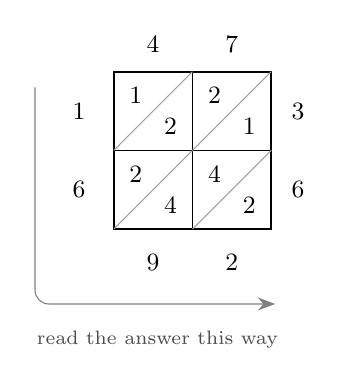
\begin{tikzpicture}[baseline=(current bounding box.north),scale=1.0]
  \lsetup{2}{2}
  \lgrid
  \ltop{1}{4} \ltop{2}{7}
  \lside{1}{3} \lside{2}{6}
  \lcell{1}{1}{1}{2} \lcell{2}{1}{2}{1}
  \lcell{1}{2}{2}{4} \lcell{2}{2}{4}{2}
  \lleft{1}{1} \lleft{2}{6}
  \lbot{1}{9} \lbot{2}{2}
  \lreadarrow
  \node[font=\scriptsize,gray!60!black,anchor=west] at (-1.1,-1.4)
    {read the answer this way};
\end{tikzpicture}
\end{minipage}%
\begin{minipage}[t]{0.56\linewidth}
\vspace{2pt}
$4\times3=12$, \; $7\times3=21$, \; $4\times6=24$, \; $7\times6=42$

\smallskip
\ealpara{Dodając \ealkeytr{przekątne}, zaczynając od prawego dolnego rogu: pierwsza \ealkeytr{przekątna}: $2=2$; druga \ealkeytr{przekątna}: $4+4+1=9$; trzecia \ealkeytr{przekątna}: $2+2+2=6$; czwarta \ealkeytr{przekątna}: $1=1$.}{Adding the \ealkey{diagonals}, starting from the bottom right corner: 1st \ealkey{diagonal}: $2=2$; 2nd \ealkey{diagonal}: $4+4+1=9$; 3rd \ealkey{diagonal}: $2+2+2=6$; 4th \ealkey{diagonal}: $1=1$.}
\vspace{-2pt}
\begin{align*}
  \text{1st diagonal:}\quad & 2 && = 2\\[-3pt]
  \text{2nd diagonal:}\quad & 4+4+1 && = 9\\[-3pt]
  \text{3rd diagonal:}\quad & 2+2+2 && = 6\\[-3pt]
  \text{4th diagonal:}\quad & 1 && = 1
\end{align*}
\vspace{-14pt}

\ealpara{Zatem $47\times36=1692$.}{So $47\times36=1692$.}
\end{minipage}
\end{wex}

\begin{enumerate}

\item \ealpara{Obie \ealkeytr{siatki} poniżej są już wypełnione. Dodaj wzdłuż \ealkeytr{przekątnych} i zapisz odpowiedź. Jedna \ealkeytr{przekątna} w części (b) sumuje się do więcej niż dziesięć, więc będziesz musiał \ealkeytr{przenosić}.}{Both \ealkey{grids} below are already filled in. Add along the \ealkey{diagonals} and write the answer. One \ealkey{diagonal} in part (b) adds up to more than ten, so you will need to \ealkey{carry}.}
\vspace{2pt}

\begin{minipage}[t]{0.5\linewidth}
\centering
(a) $52\times34$\\[4pt]
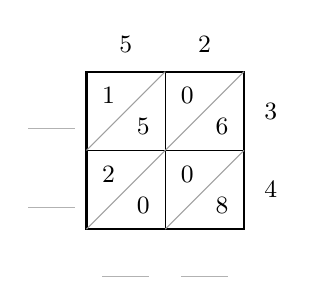
\begin{tikzpicture}[baseline=(current bounding box.north),scale=1.0]
  \lsetup{2}{2}
  \lgrid
  \ltop{1}{5} \ltop{2}{2}
  \lside{1}{3} \lside{2}{4}
  \lcell{1}{1}{1}{5} \lcell{2}{1}{0}{6}
  \lcell{1}{2}{2}{0} \lcell{2}{2}{0}{8}
  \lanslines
\end{tikzpicture}\\[8pt]
$52\times34=\ansline[2cm]$
\end{minipage}%
\begin{minipage}[t]{0.5\linewidth}
\centering
(b) $68\times47$\\[4pt]
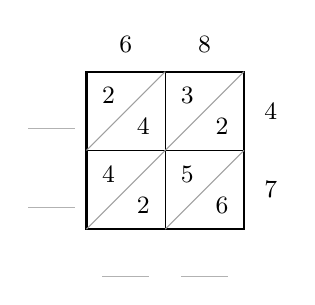
\begin{tikzpicture}[baseline=(current bounding box.north),scale=1.0]
  \lsetup{2}{2}
  \lgrid
  \ltop{1}{6} \ltop{2}{8}
  \lside{1}{4} \lside{2}{7}
  \lcell{1}{1}{2}{4} \lcell{2}{1}{3}{2}
  \lcell{1}{2}{4}{2} \lcell{2}{2}{5}{6}
  \lanslines
\end{tikzpicture}\\[8pt]
$68\times47=\ansline[2cm]$
\end{minipage}

\newpage

\item \ealpara{Te \ealkeytr{siatki} są narysowane, ale puste. Wypełnij każdą \ealkeytr{komórkę}, a następnie dodaj wzdłuż \ealkeytr{przekątnych}. Część (b) ma liczbę składającą się z trzech \ealkeytr{cyfr}, więc jej \ealkeytr{siatka} ma trzy \ealkeytr{kolumny}.}{These \ealkey{grids} are drawn but empty. Fill in every \ealkey{cell}, then add along the \ealkey{diagonals}. Part (b) has a three-\ealkey{digit} number, so its \ealkey{grid} has three \ealkey{columns}.}
\vspace{2pt}

\begin{minipage}[t]{0.42\linewidth}
\centering
(a) $34\times25$\\[4pt]
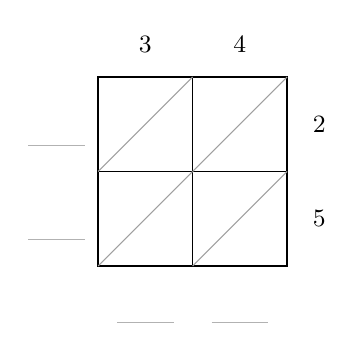
\begin{tikzpicture}[baseline=(current bounding box.north),scale=1.2]
  \lsetup{2}{2}
  \lgrid
  \ltop{1}{3} \ltop{2}{4}
  \lside{1}{2} \lside{2}{5}
  \lanslines
\end{tikzpicture}\\[8pt]
$34\times25=\ansline[2cm]$
\end{minipage}%
\begin{minipage}[t]{0.58\linewidth}
\centering
(b) $243\times17$\\[4pt]
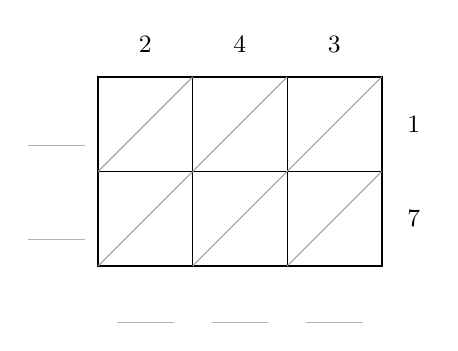
\begin{tikzpicture}[baseline=(current bounding box.north),scale=1.2]
  \lsetup{3}{2}
  \lgrid
  \ltop{1}{2} \ltop{2}{4} \ltop{3}{3}
  \lside{1}{1} \lside{2}{7}
  \lanslines
\end{tikzpicture}\\[8pt]
$243\times17=\ansline[2cm]$
\end{minipage}

\end{enumerate}

\ealpara{Gdzie trafia \ealkeytr{przecinek dziesiętny}}{Where the \ealkey{decimal point} goes}
\parttitle{2}{Where the \ealkey{decimal point} goes}

\ealpara{Metodę \ealkeytr{kratową} można również stosować do \ealkeytr{mnożenia} \ealkeytr{liczb dziesiętnych}. \ealkeytr{Przecinek dziesiętny} w odpowiedzi znajduje się na \ealkeytr{przekątnej}, na której spotykają się dwa \ealkeytr{przecinki dziesiętne} w mnożonych liczbach, jak pokazano poniżej.}{The \ealkey{lattice} method can also be used to \ealkey{multiply} \ealkey{decimal numbers}. The \ealkey{decimal point} in the answer is located on the \ealkey{diagonal} where the two \ealkey{decimal points} in the numbers being multiplied meet, as seen below.}

\begin{wex}{$2.6\times3.4$}
\small
\begin{minipage}[t]{0.40\linewidth}
\centering
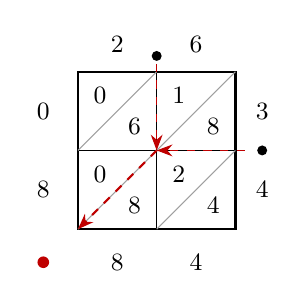
\begin{tikzpicture}[baseline=(current bounding box.north),scale=1.0]
  \lsetup{2}{2}
  \lgrid
  \ltop{1}{2} \ltop{2}{6} \ltopdot{1}
  \lside{1}{3} \lside{2}{4} \lsidedot{1}
  \lcell{1}{1}{0}{6} \lcell{2}{1}{1}{8}
  \lcell{1}{2}{0}{8} \lcell{2}{2}{2}{4}
  \lleft{1}{0} \lleft{2}{8}
  \lbot{1}{8} \lbot{2}{4}
  \ltrace{1}{1}
\end{tikzpicture}
\end{minipage}%
\begin{minipage}[t]{0.60\linewidth}
\vspace{2pt}
\ealpara{\ealkeytr{Cyfry} wzdłuż góry to $2$ i $6$, z \ealkeytr{przecinkiem dziesiętnym} po pierwszej z nich. \ealkeytr{Cyfry} wzdłuż boku to $3$ i $4$, znów z \ealkeytr{przecinkiem dziesiętnym} po pierwszej z nich.}{The \ealkey{digits} along the top are $2$ and $6$, with the \ealkey{decimal point} after the first of them. The \ealkey{digits} down the side are $3$ and $4$, again with the \ealkey{decimal point} after the first of them.}

\smallskip
\ealpara{Dodając \ealkeytr{przekątne} od prawego dolnego rogu, otrzymujemy $4$, potem $2+8+8=18$, więc zapisujemy $8$ i \ealkeytr{przenosimy} $1$, potem $0+1+6+1=8$, potem $0$.}{Adding the \ealkey{diagonals} from the bottom right corner gives $4$, then $2+8+8=18$, so we write $8$ and \ealkey{carry} $1$, then $0+1+6+1=8$, then $0$.}

\smallskip
\ealpara{Dwie przerywane linie spotykają się w środku \ealkeytr{siatki}, a \ealkeytr{przekątna} stamtąd opuszcza \ealkeytr{siatkę} w lewym dolnym rogu. Zatem \ealkeytr{cyfry} $0884$ stają się $08.84$, co zapisujemy jako $8.84$.}{The two dashed lines meet in the middle of the \ealkey{grid}, and the \ealkey{diagonal} from there leaves the \ealkey{grid} at the bottom left corner. So the \ealkey{digits} $0884$ become $08.84$, which we write as $8.84$.}
\end{minipage}
\end{wex}

\begin{enumerate}[resume]

\newpage

\item \ealpara{Ta \ealkeytr{siatka} jest już wypełniona. Dodaj wzdłuż \ealkeytr{przekątnych}, a następnie użyj \ealkeytr{przecinków dziesiętnych} zaznaczonych na \ealkeytr{siatce}, aby ustalić, gdzie w odpowiedzi znajduje się \ealkeytr{przecinek dziesiętny}.}{This \ealkey{grid} is already filled in. Add along the \ealkey{diagonals}, then use the \ealkey{decimal points} marked on the \ealkey{grid} to work out where the \ealkey{decimal point} goes in the answer.}
\vspace{2pt}

\begin{center}
\begin{minipage}[t]{0.44\linewidth}
\centering
$1.7\times4.3$\\[4pt]
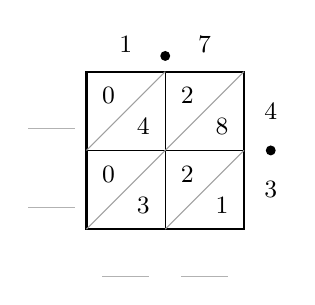
\begin{tikzpicture}[baseline=(current bounding box.north),scale=1.0]
  \lsetup{2}{2}
  \lgrid
  \ltop{1}{1} \ltop{2}{7} \ltopdot{1}
  \lside{1}{4} \lside{2}{3} \lsidedot{1}
  \lcell{1}{1}{0}{4} \lcell{2}{1}{2}{8}
  \lcell{1}{2}{0}{3} \lcell{2}{2}{2}{1}
  \lanslines
\end{tikzpicture}\\[8pt]
$1.7\times4.3=\ansline[2cm]$
\end{minipage}
\end{center}

\item \ealpara{Wypełnij te \ealkeytr{siatki}, a następnie ustal, gdzie znajduje się \ealkeytr{przecinek dziesiętny}. W części (b) \ealkeytr{przecinki dziesiętne} nie są w tym samym miejscu w obu liczbach, więc dwie linie nie spotkają się w środku \ealkeytr{siatki}.}{Fill in these \ealkey{grids}, then find where the \ealkey{decimal point} goes. In part (b) the \ealkey{decimal points} are not in the same place in the two numbers, so the two lines will not meet in the middle of the \ealkey{grid}.}
\vspace{2pt}

\begin{minipage}[t]{0.42\linewidth}
\centering
(a) $0.6\times4.5$\\[4pt]
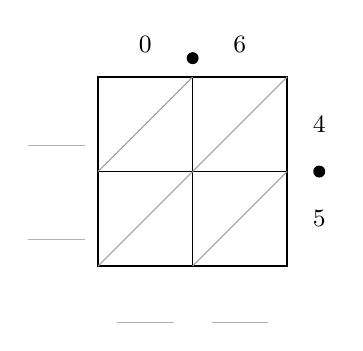
\begin{tikzpicture}[baseline=(current bounding box.north),scale=1.2]
  \lsetup{2}{2}
  \lgrid
  \ltop{1}{0} \ltop{2}{6} \ltopdot{1}
  \lside{1}{4} \lside{2}{5} \lsidedot{1}
  \lanslines
\end{tikzpicture}\\[8pt]
$0.6\times4.5=\ansline[2cm]$
\end{minipage}%
\begin{minipage}[t]{0.58\linewidth}
\centering
(b) $12.4\times0.3$\\[4pt]
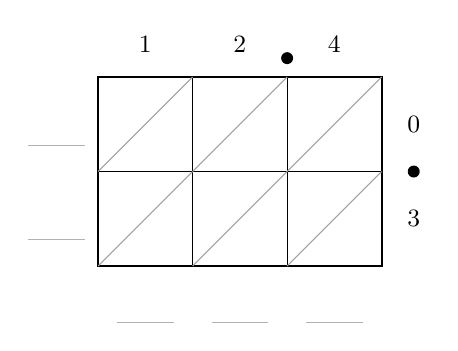
\begin{tikzpicture}[baseline=(current bounding box.north),scale=1.2]
  \lsetup{3}{2}
  \lgrid
  \ltop{1}{1} \ltop{2}{2} \ltop{3}{4} \ltopdot{2}
  \lside{1}{0} \lside{2}{3} \lsidedot{1}
  \lanslines
\end{tikzpicture}\\[8pt]
$12.4\times0.3=\ansline[2cm]$
\end{minipage}

\item \ealpara{Użyj swojej odpowiedzi do Q4 część (a), aby zapisać każdy z tych przykładów bez rysowania \ealkeytr{siatki}. Wyjaśnij, jak zdecydowałeś, gdzie za każdym razem umieścić \ealkeytr{przecinek dziesiętny}.}{Use your answer to Q4 part (a) to write down each of these without drawing a \ealkey{grid}. Explain how you decided where to put the \ealkey{decimal point} each time.}
\begin{multicols}{3}
\begin{enumerate}
  \item $6\times45=\ansline[1.5cm]$
  \item $0.06\times4.5=\ansline[1.5cm]$
  \item $60\times0.45=\ansline[1.5cm]$
\end{enumerate}
\end{multicols}
\vspace{13em}

\end{enumerate}

\newpage

\ealpara{Korzystanie z metody}{Using the method}
\parttitle{3}{Using the method}

\ealpara{\ealkeytr{Przecinek dziesiętny} \ealkeytr{liczby całkowitej nieujemnej} znajduje się na końcu jej \ealkeytr{cyfr}, więc jego znacznik trafia na róg \ealkeytr{siatki}. Wszystko inne w tej metodzie pozostaje bez zmian.}{The \ealkey{decimal point} of a \ealkey{whole number} is at the end of its \ealkey{digits}, so its mark goes on the corner of the \ealkey{grid}. Everything else about the method stays the same.}

\begin{enumerate}[resume]

\item
\begin{enumerate}
  \item \ealpara{Szkoła zamawia $24$ paczki ołówków. Każda paczka kosztuje \pounds3.65. Użyj \ealkeytr{siatki}, aby obliczyć całkowity koszt zamówienia.}{A school orders $24$ packs of pencils. Each pack costs \pounds3.65. Use the \ealkey{grid} to work out the total cost of the order.}
        \vspace{2pt}

        \begin{center}
        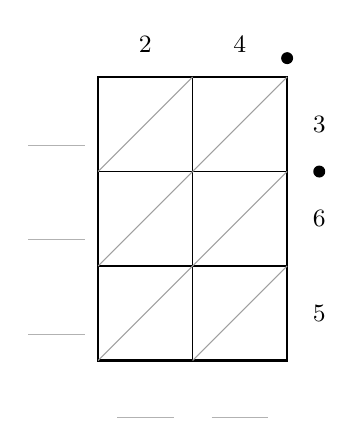
\begin{tikzpicture}[baseline=(current bounding box.north),scale=1.2]
          \lsetup{2}{3}
          \lgrid
          \ltop{1}{2} \ltop{2}{4} \ltopdot{2}
          \lside{1}{3} \lside{2}{6} \lside{3}{5} \lsidedot{1}
          \lanslines
        \end{tikzpicture}
        \end{center}
        \vspace{2pt}
        \ealpara{Całkowity koszt: \pounds\ansline[2.5cm]}{Total cost: \pounds\ansline[2.5cm]}

  \item \ealpara{Cieknący kran traci $0.35$ litra wody co godzinę. Użyj \ealkeytr{siatki}, aby obliczyć, ile wody traci w ciągu $16$ godzin.}{A dripping tap loses $0.35$ litres of water every hour. Use the \ealkey{grid} to work out how much water it loses in $16$ hours.}
        \vspace{2pt}

        \begin{center}
        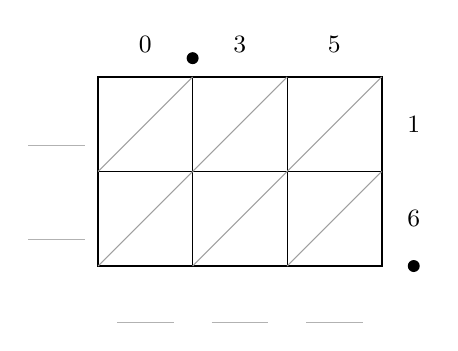
\begin{tikzpicture}[baseline=(current bounding box.north),scale=1.2]
          \lsetup{3}{2}
          \lgrid
          \ltop{1}{0} \ltop{2}{3} \ltop{3}{5} \ltopdot{1}
          \lside{1}{1} \lside{2}{6} \lsidedot{2}
          \lanslines
        \end{tikzpicture}
        \end{center}
        \vspace{2pt}
        \ealpara{Utracona woda: \ansline[2.5cm] litrów}{Water lost: \ansline[2.5cm] litres}
\end{enumerate}

\newpage

\item \ealpara{Narysuj własną \ealkeytr{siatkę} dla każdego z tych przykładów. Zaznacz \ealkeytr{przecinki dziesiętne} na krawędziach \ealkeytr{siatki} i pokaż \ealkeytr{przekątną}, którą podążałeś, aby umieścić \ealkeytr{przecinek dziesiętny} w odpowiedzi.}{Draw your own \ealkey{grid} for each of these. Mark the \ealkey{decimal points} on the edges of the \ealkey{grid}, and show the \ealkey{diagonal} you followed to place the \ealkey{decimal point} in the answer.}
\vspace{2pt}

\begin{minipage}[t]{0.46\linewidth}
\ealpara{(a) Benzyna kosztuje \pounds1.45 za litr. Kofi kupuje $38$ litrów. Ile płaci?}{(a) Petrol costs \pounds1.45 per litre. Kofi buys $38$ litres. How much does he pay?}

\vspace{13em}
\end{minipage}\hfill
\begin{minipage}[t]{0.46\linewidth}
\ealpara{(b) \ealkeytr{Prostokątna} płytka ma wymiary $4.8$ cm na $2.5$ cm. Jakie jest jej \ealkeytr{pole}?}{(b) A \ealkey{rectangular} tile measures $4.8$ cm by $2.5$ cm. What is its \ealkey{area}?}

\vspace{13em}
\end{minipage}

\item \ealpara{\textbf{Praktyka.} Użyj chińskiej metody \ealkeytr{mnożenia} dla każdego z tych przykładów, samodzielnie rysując \ealkeytr{siatki}.}{\textbf{Practice.} Use the Chinese \ealkey{multiplication} method for each of these, drawing the \ealkey{grids} yourself.}
\begin{multicols}{3}
\begin{enumerate}
  \item $73\times48$
  \item $5.2\times3.6$
  \item $0.9\times0.7$
  \item $126\times34$
  \item $8.4\times0.25$
  \item $1.06\times3.5$
\end{enumerate}
\end{multicols}
\vspace{26em}

\end{enumerate}

\newpage

\ealpara{Wyzwania}{Challenges}
\parttitle{4}{Challenges}

\begin{enumerate}[resume]

\item \ealpara{\textbf{Dlaczego \ealkeytr{przekątne} działają.} W \ealkeytr{siatce} dla $47\times36$ \ealkeytr{komórka} zawierająca $4\times6$ i \ealkeytr{komórka} zawierająca $7\times3$ leżą na tej samej \ealkeytr{przekątnej}.}{\textbf{Why the \ealkey{diagonals} work.} In the \ealkey{grid} for $47\times36$, the \ealkey{cell} holding $4\times6$ and the \ealkey{cell} holding $7\times3$ lie on the same \ealkey{diagonal}.}
\begin{enumerate}
  \item \ealpara{Oblicz $40\times6$ i $7\times30$. Co zauważasz w obu odpowiedziach?}{Work out $40\times6$ and $7\times30$. What do you notice about the two answers?}

        \vspace{6.5em}
  \item \ealpara{Użyj części (a), aby wyjaśnić, dlaczego dwie \ealkeytr{komórki} na tej \ealkeytr{przekątnej} są dodawane do siebie.}{Use part (a) to explain why the two \ealkey{cells} on that \ealkey{diagonal} are added together.}

        \vspace{7.5em}
\end{enumerate}

\item \ealpara{Sam używa tej metody dla $0.48\times0.25$. Jego \ealkeytr{cyfry} wychodzą jako $001200$ i zapisuje odpowiedź $1200$.}{Sam uses the method on $0.48\times0.25$. His \ealkey{digits} come out as $001200$, and he writes the answer $1200$.}
\begin{enumerate}
  \item \ealpara{Bez wykonywania \ealkeytr{mnożenia}, wyjaśnij, skąd wiesz, że $1200$ nie może być poprawne.}{Without working the \ealkey{multiplication} out, explain how you know that $1200$ cannot be right.}

        \vspace{5.5em}
  \item \ealpara{Narysuj \ealkeytr{siatkę}, umieść \ealkeytr{przecinek dziesiętny} i zapisz poprawną odpowiedź.}{Draw the \ealkey{grid}, place the \ealkey{decimal point}, and write down the correct answer.}

        \vspace{14em}
\end{enumerate}

\newpage

\item \ealpara{Ile \ealkeytr{mnożeń} pojedynczych \ealkeytr{cyfr} potrzeba, aby obliczyć liczbę składającą się z trzech \ealkeytr{cyfr} \ealkeytr{pomnożoną} przez liczbę składającą się z czterech \ealkeytr{cyfr}? Wyjaśnij, skąd to wiesz, bez rysowania \ealkeytr{siatki}.}{How many single-\ealkey{digit} \ealkey{multiplications} does the method need to work out a three-\ealkey{digit} number \ealkey{multiplied} by a four-\ealkey{digit} number? Explain how you know without drawing the \ealkey{grid}.}

\vspace{9em}

\item \ealpara{Zaprojektuj \ealkeytr{mnożenie} dwóch liczb, z których każda jest zapisana z dokładnością do jednego \ealkeytr{miejsca dziesiętnego}, którego wynik wynosi dokładnie $0.36$. Pokaż, że twoje \ealkeytr{mnożenie} działa, używając chińskiej metody \ealkeytr{mnożenia}.}{Design a \ealkey{multiplication} of two numbers, each written to one \ealkey{decimal place}, whose answer is exactly $0.36$. Show that your \ealkey{multiplication} works using the Chinese \ealkey{multiplication} method.}

\vspace{18em}

\item \ealpara{Zainab mówi: „Chińska metoda \ealkeytr{mnożenia} jest lepsza od \ealkeytr{metody kolumnowej}, ponieważ nigdy nie musisz \ealkeytr{przenosić}.” Użyj jednej ze swoich odpowiedzi z tej karty, aby zdecydować, czy ma rację.}{Zainab says: ``The Chinese \ealkey{multiplication} method is better than the \ealkey{column method}, because you never have to \ealkey{carry}.'' Use one of your answers from this sheet to decide whether she is right.}

\vspace{13em}

\end{enumerate}

\newpage

\ealpara{Odpowiedzi}{Answers}
\heading{Answers}

{\small
\begin{multicols}{2}
\raggedcolumns
\setlength{\parskip}{4pt}

\ealpara{\textbf{Q1.} (a) \ealkeytr{Przekątne} dają $8$, potem $0+0+6=6$, potem $2+0+5=7$, potem $1$, więc $52\times34=1768$. \quad (b) \ealkeytr{Przekątne} dają $6$, potem $5+2+2=9$, potem $4+3+4=11$, więc zapisujemy $1$ i \ealkeytr{przenosimy} $1$, potem $2+1=3$, więc $68\times47=3196$.}{\textbf{Q1.} (a) The \ealkey{diagonals} give $8$, then $0+0+6=6$, then $2+0+5=7$, then $1$, so $52\times34=1768$. \quad (b) The \ealkey{diagonals} give $6$, then $5+2+2=9$, then $4+3+4=11$, so write $1$ and \ealkey{carry} $1$, then $2+1=3$, so $68\times47=3196$.}

\ealpara{\textbf{Q2.} (a) \ealkeytr{Komórki} zawierają $06$, $08$, $15$ i $20$. \ealkeytr{Przekątne} dają $0$, potem $2+5+8=15$, więc zapisujemy $5$ i \ealkeytr{przenosimy} $1$, potem $1+0+6+1=8$, potem $0$, więc $34\times25=850$. \quad (b) \ealkeytr{Komórki} zawierają $02$, $04$ i $03$ wzdłuż górnego \ealkeytr{wiersza}, oraz $14$, $28$ i $21$ wzdłuż dolnego \ealkeytr{wiersza}. \ealkeytr{Przekątne} dają $1$, potem $2+8+3=13$, potem $2+4+4+0+1=11$, potem $1+0+2+1=4$, potem $0$, więc $243\times17=4131$.}{\textbf{Q2.} (a) The \ealkey{cells} hold $06$, $08$, $15$ and $20$. The \ealkey{diagonals} give $0$, then $2+5+8=15$, so write $5$ and \ealkey{carry} $1$, then $1+0+6+1=8$, then $0$, so $34\times25=850$. \quad (b) The \ealkey{cells} hold $02$, $04$ and $03$ along the top \ealkey{row}, and $14$, $28$ and $21$ along the bottom \ealkey{row}. The \ealkey{diagonals} give $1$, then $2+8+3=13$, then $2+4+4+0+1=11$, then $1+0+2+1=4$, then $0$, so $243\times17=4131$.}

\ealpara{\textbf{Q3.} \ealkeytr{Cyfry} to $0731$. Oba \ealkeytr{przecinki dziesiętne} znajdują się po pierwszej \ealkeytr{cyfrze} swojej liczby, więc dwie linie spotykają się w środku \ealkeytr{siatki}, a \ealkeytr{przekątna} opuszcza \ealkeytr{siatkę} w lewym dolnym rogu: $07.31$, czyli $7.31$.}{\textbf{Q3.} The \ealkey{digits} are $0731$. Both \ealkey{decimal points} sit after the first \ealkey{digit} of their number, so the two lines meet in the middle of the \ealkey{grid} and the \ealkey{diagonal} leaves the \ealkey{grid} at the bottom left corner: $07.31$, which is $7.31$.}

\ealpara{\textbf{Q4.} (a) \ealkeytr{Komórki} zawierają $00$, $24$, $00$ i $30$. \ealkeytr{Cyfry} to $0270$, a \ealkeytr{przekątna} opuszcza \ealkeytr{siatkę} w lewym dolnym rogu, dając $02.70$, więc $0.6\times4.5=2.7$. \quad (b) \ealkeytr{Komórki} zawierają $00$, $00$ i $00$ wzdłuż górnego \ealkeytr{wiersza}, oraz $03$, $06$ i $12$ wzdłuż dolnego \ealkeytr{wiersza}. \ealkeytr{Cyfry} to $00372$. Linia w dół od góry spotyka linię wchodzącą z boku o jedną \ealkeytr{kolumnę} dalej w prawo, więc \ealkeytr{przekątna} opuszcza \ealkeytr{siatkę} przez dolną krawędź, między trzecią a czwartą \ealkeytr{cyfrą}: $003.72$, więc $12.4\times0.3=3.72$.}{\textbf{Q4.} (a) The \ealkey{cells} hold $00$, $24$, $00$ and $30$. The \ealkey{digits} are $0270$ and the \ealkey{diagonal} leaves the \ealkey{grid} at the bottom left corner, giving $02.70$, so $0.6\times4.5=2.7$. \quad (b) The \ealkey{cells} hold $00$, $00$ and $00$ along the top \ealkey{row}, and $03$, $06$ and $12$ along the bottom \ealkey{row}. The \ealkey{digits} are $00372$. The line down from the top meets the line in from the side one \ealkey{column} further to the right, so the \ealkey{diagonal} leaves the \ealkey{grid} through the bottom edge, between the third and fourth \ealkey{digits}: $003.72$, so $12.4\times0.3=3.72$.}

\ealpara{\textbf{Q5.} (a) $270$ \quad (b) $0.27$ \quad (c) $27$. \ealkeytr{Cyfry} odpowiedzi to $27$ za każdym razem, ponieważ \ealkeytr{cyfry}, które są \ealkeytr{mnożone}, nie zmieniły się. Zmienia się tylko \ealkeytr{wartość pozycyjna}: w (a) obie liczby zostały \ealkeytr{pomnożone} przez $10$, więc odpowiedź jest $100$ razy większa niż $2.7$; w (b) pierwsza liczba została podzielona przez $10$, więc odpowiedź jest $10$ razy mniejsza; w (c) pierwsza liczba została \ealkeytr{pomnożona} przez $100$, a druga podzielona przez $10$, więc odpowiedź jest $10$ razy większa.}{\textbf{Q5.} (a) $270$ \quad (b) $0.27$ \quad (c) $27$. The \ealkey{digits} of the answer are $27$ every time, because the \ealkey{digits} being \ealkey{multiplied} have not changed. Only the \ealkey{place value} changes: in (a) both numbers have been \ealkey{multiplied} by $10$, so the answer is $100$ times larger than $2.7$; in (b) the first number has been divided by $10$, so the answer is $10$ times smaller; in (c) the first number has been \ealkey{multiplied} by $100$ and the second divided by $10$, so the answer is $10$ times larger.}

\ealpara{\textbf{Q6.} (a) \ealkeytr{Cyfry} to $08760$. \ealkeytr{Przecinek dziesiętny} liczby $24$ znajduje się w prawym rogu \ealkeytr{siatki}, a \ealkeytr{przekątna} od miejsca spotkania dwóch linii opuszcza \ealkeytr{siatkę} w lewym dolnym rogu, dając $087.60$. Zamówienie kosztuje \pounds$87.60$. \quad (b) \ealkeytr{Cyfry} to $00560$, a \ealkeytr{przecinek dziesiętny} znajduje się między trzecią a czwartą z nich, dając $005.60$. Kran traci $5.6$ litra.}{\textbf{Q6.} (a) The \ealkey{digits} are $08760$. The \ealkey{decimal point} of $24$ is on the right-hand corner of the \ealkey{grid}, and the \ealkey{diagonal} from where the two lines meet leaves the \ealkey{grid} at the bottom left corner, giving $087.60$. The order costs \pounds$87.60$. \quad (b) The \ealkey{digits} are $00560$, and the \ealkey{decimal point} goes between the third and fourth of them, giving $005.60$. The tap loses $5.6$ litres.}

\ealpara{\textbf{Q7.} (a) $1.45\times38=55.10$, więc Kofi płaci \pounds$55.10$. \quad (b) $4.8\times2.5=12.00$, więc \ealkeytr{pole} wynosi $12$ cm$^2$. Dwa zera po \ealkeytr{przecinku dziesiętnym} nie zmieniają wartości, więc nie są zapisywane.}{\textbf{Q7.} (a) $1.45\times38=55.10$, so Kofi pays \pounds$55.10$. \quad (b) $4.8\times2.5=12.00$, so the \ealkey{area} is $12$ cm$^2$. The two zeros after the \ealkey{decimal point} do not change the value, so they are not written.}

\textbf{Q8.} (a) $3504$ \quad (b) $18.72$ \quad (c) $0.63$ \quad (d) $4284$ \quad (e) $2.1$ \quad (f) $3.71$

\ealpara{\textbf{Q9.} (a) $40\times6=240$ i $7\times30=210$. Obie odpowiedzi to \ealkeytr{liczba całkowita nieujemna} dziesiątek, więc \ealkeytr{cyfra}, którą każda z nich wnosi, trafia do \ealkeytr{kolumny} dziesiątek w odpowiedzi. \quad (b) \ealkeytr{Komórka} tak naprawdę nie zawiera $4\times6$; zawiera $40\times6$, ponieważ $4$ jest w \ealkeytr{kolumnie} dziesiątek. Każda \ealkeytr{komórka} na tej samej \ealkeytr{przekątnej} oznacza tę samą \ealkeytr{wartość pozycyjną} w odpowiedzi, dlatego \ealkeytr{cyfry} na jednej \ealkeytr{przekątnej} są dodawane do siebie i dlatego \ealkeytr{przekątna} sumująca się do dziesięciu lub więcej \ealkeytr{przenosi} do następnej \ealkeytr{przekątnej}.}{\textbf{Q9.} (a) $40\times6=240$ and $7\times30=210$. Both answers are a \ealkey{whole number} of tens, so the \ealkey{digit} each one contributes lands in the tens \ealkey{column} of the answer. \quad (b) A \ealkey{cell} does not really hold $4\times6$; it holds $40\times6$, because the $4$ is in the tens \ealkey{column}. Every \ealkey{cell} on the same \ealkey{diagonal} stands for the same \ealkey{place value} in the answer, which is why the \ealkey{digits} on one \ealkey{diagonal} are added together, and why a \ealkey{diagonal} totalling ten or more \ealkey{carries} into the next \ealkey{diagonal}.}

\ealpara{\textbf{Q10.} (a) $0.48$ jest mniejsze niż $1$, a $0.25$ jest mniejsze niż $1$, więc odpowiedź musi być mniejsza niż którakolwiek z nich, a z pewnością mniejsza niż $1$. Odpowiedź Sama jest większa niż tysiąc. \quad (b) \ealkeytr{Cyfry} to $001200$. \ealkeytr{Przecinek dziesiętny} liczby $0.48$ znajduje się po jej pierwszej \ealkeytr{kolumnie}, a \ealkeytr{przecinek dziesiętny} liczby $0.25$ po jej pierwszym \ealkeytr{wierszu}, więc dwie linie spotykają się o jedną \ealkeytr{komórkę} od lewego górnego rogu. \ealkeytr{Przekątna} stamtąd opuszcza \ealkeytr{siatkę} przez lewą stronę, między drugą a trzecią \ealkeytr{cyfrą}, dając $00.1200$. Zatem $0.48\times0.25=0.12$.}{\textbf{Q10.} (a) $0.48$ is less than $1$ and $0.25$ is less than $1$, so the answer must be smaller than either of them, and certainly smaller than $1$. Sam's answer is more than a thousand. \quad (b) The \ealkey{digits} are $001200$. The \ealkey{decimal point} of $0.48$ is after its first \ealkey{column} and the \ealkey{decimal point} of $0.25$ is after its first \ealkey{row}, so the two lines meet one \ealkey{cell} in from the top left corner. The \ealkey{diagonal} from there leaves the \ealkey{grid} through the left-hand side, between the second and third \ealkey{digits}, giving $00.1200$. So $0.48\times0.25=0.12$.}

\ealpara{\textbf{Q11.} $12$ \ealkeytr{mnożeń}. \ealkeytr{Siatka} ma jedną \ealkeytr{kolumnę} dla każdej z trzech \ealkeytr{cyfr} i jeden \ealkeytr{wiersz} dla każdej z czterech \ealkeytr{cyfr}, więc ma $3\times4=12$ \ealkeytr{komórek}, a każda \ealkeytr{komórka} zawiera jedno \ealkeytr{mnożenie} pojedynczych \ealkeytr{cyfr}.}{\textbf{Q11.} $12$ \ealkey{multiplications}. The \ealkey{grid} has one \ealkey{column} for each of the three \ealkey{digits} and one \ealkey{row} for each of the four \ealkey{digits}, so it has $3\times4=12$ \ealkey{cells}, and each \ealkey{cell} holds one single-\ealkey{digit} \ealkey{multiplication}.}

\ealpara{\textbf{Q12.} Wiele odpowiedzi. Na przykład $0.4\times0.9$, $0.6\times0.6$, $1.2\times0.3$ i $1.8\times0.2$ dają $0.36$. \ealkeytr{Cyfry} dwóch liczb muszą \ealkeytr{mnożyć} się do $36$, a każda liczba ma jedną \ealkeytr{cyfrę} po \ealkeytr{przecinku dziesiętnym}, więc odpowiedź ma dwie.}{\textbf{Q12.} Many answers. For example $0.4\times0.9$, $0.6\times0.6$, $1.2\times0.3$ and $1.8\times0.2$ all give $0.36$. The \ealkey{digits} of the two numbers have to \ealkey{multiply} to $36$, and each number has one \ealkey{digit} after the \ealkey{decimal point}, so the answer has two.}

\ealpara{\textbf{Q13.} Ma częściowo rację. Podczas wypełniania \ealkeytr{siatki} nie zachodzi żadne \ealkeytr{przenoszenie}, ponieważ każda \ealkeytr{komórka} zawiera \ealkeytr{mnożenie} pojedynczych \ealkeytr{cyfr}, a jej dwie \ealkeytr{cyfry} mają po jednym trójkącie. \ealkeytr{Przenoszenie} nadal zachodzi, gdy dodawane są \ealkeytr{przekątne}: w Q1 część (b) trzecia \ealkeytr{przekątna} dała $11$, więc $1$ trzeba było \ealkeytr{przenieść} do następnej \ealkeytr{przekątnej}.}{\textbf{Q13.} She is partly right. No \ealkey{carrying} happens while the \ealkey{grid} is being filled in, because every \ealkey{cell} holds a single-\ealkey{digit} \ealkey{multiplication} and its two \ealkey{digits} have a triangle each. \ealkey{Carrying} does still happen when the \ealkey{diagonals} are added: in Q1 part (b) the third \ealkey{diagonal} came to $11$, so the $1$ had to be \ealkey{carried} into the next \ealkey{diagonal}.}

\end{multicols}
}

\end{document}